\section{Simulazione SITL}

\begin{lstlisting}
###sil.sh
#!/bin/bash

export GAZEBO_MODEL_DATABASE_URI=""

sim=$1

Firmware=$(realpath .)

#cp posix-configs/SITL/init/ekf2/iris posix-configs/SITL/init/ekf2/sim

if [ "$#" -lt 1 ]
then
echo Specificare il simulatore : jmavsim , gazebo
exit 1
fi

if [ "$sim" == "gazebo" ] 
then
cd build/posix_sitl_default/build_gazebo
if [ "$(ls -A .)" ]
then
echo "Makefile già presente"
else
echo "Creazione makefile"
cmake $Firmware/Tools/sitl_gazebo
fi
echo "Esecuzione makefile"
make
cd $Firmware/build/posix_sitl_default
else
cd $Firmware/build/posix_sitl_default
fi



$Firmware/Tools/sitl_run.sh $Firmware/build/posix_sitl_default/px4  posix-configs/SITL/init/ekf2 none $sim sim $Firmware $Firmware/build/posix_sitl_default
\end{lstlisting}

\subsection{PID}
\subsubsection{STEP}
\todo[inline]{Tabella dei waypoints}
\begin{figure}
	\centering
	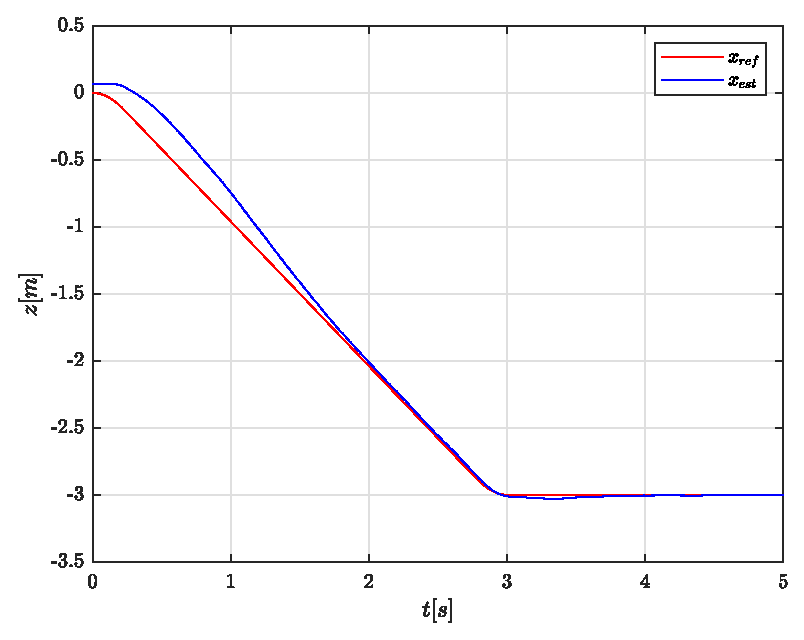
\includegraphics[width=0.5\textwidth]{Simulazioni/Figure/PID/STEP/AltitudeControlPos}
	\caption{Risposta con PID al segnale STEP : quota}
\end{figure}

\begin{figure}
	\centering
	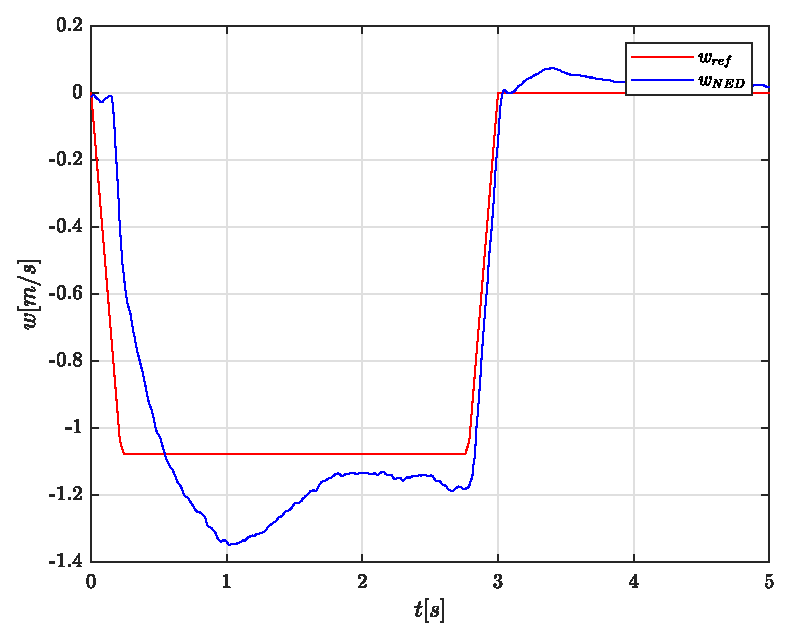
\includegraphics[width=0.5\textwidth]{Simulazioni/Figure/PID/STEP/AltitudeControlVel}
	\caption{Risposta con PID al segnale STEP : rateo di salita}
\end{figure}

\begin{figure}
	\centering
	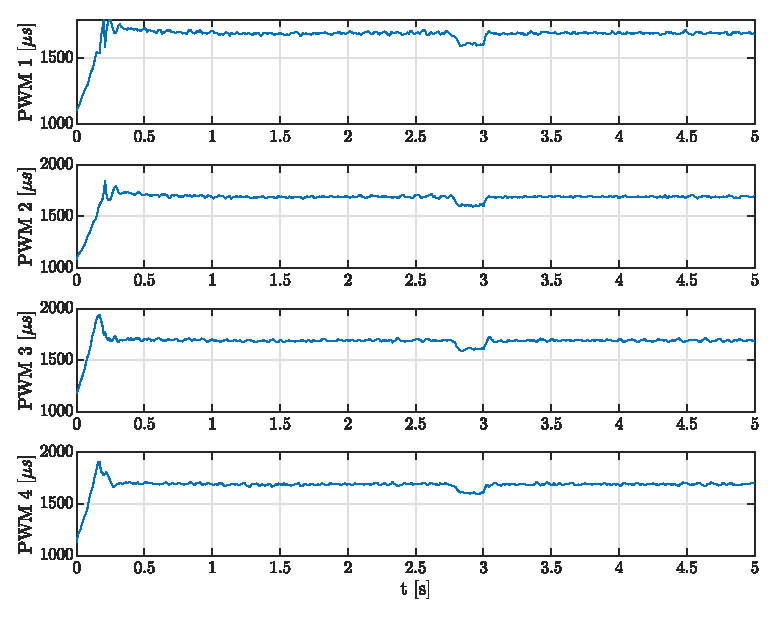
\includegraphics[width=0.5\textwidth]{Simulazioni/Figure/PID/STEP/PWM}
	\caption{Risposta con PID al segnale STEP : PWM}
\end{figure}

\clearpage
\subsection{SMC}
\subsubsection{STEP}
\todo[inline]{Tabella dei waypoints}
\begin{figure}
	\centering
	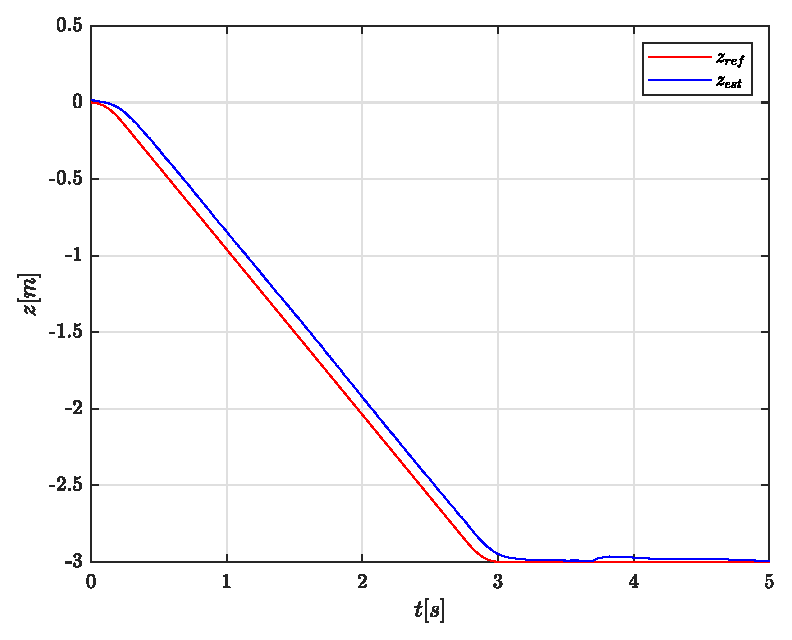
\includegraphics[width=0.5\textwidth]{Simulazioni/Figure/SMC/STEP/AltitudeControlPos}
	\caption{Risposta con PID al segnale STEP : quota}
\end{figure}

\begin{figure}
	\centering
	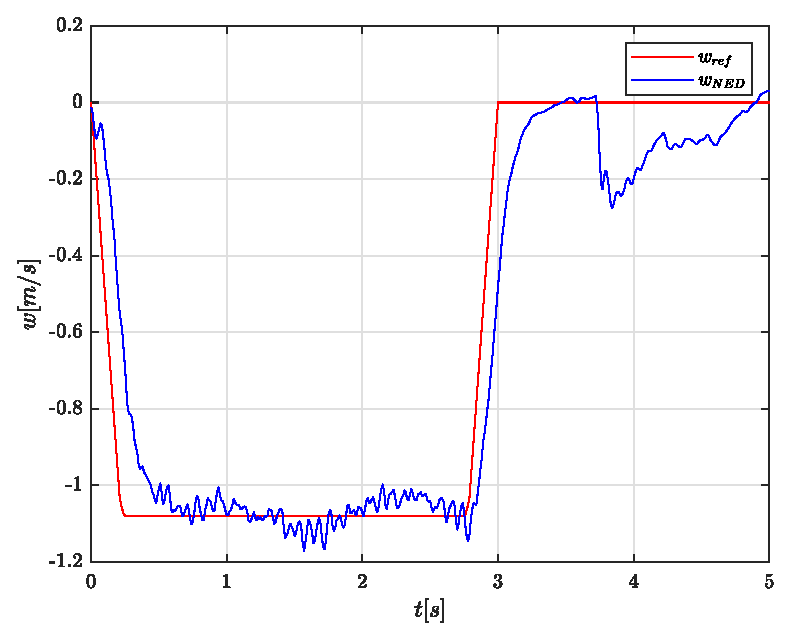
\includegraphics[width=0.5\textwidth]{Simulazioni/Figure/SMC/STEP/AltitudeControlVel}
	\caption{Risposta con PID al segnale STEP : rateo di salita}
\end{figure}

\begin{figure}
	\centering
	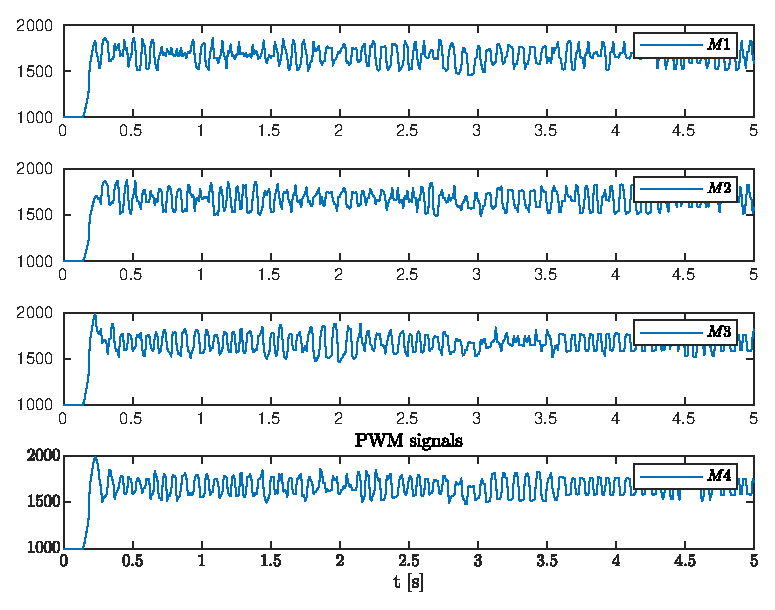
\includegraphics[width=0.5\textwidth]{Simulazioni/Figure/SMC/STEP/PWM}
	\caption{Risposta con PID al segnale STEP : PWM}
\end{figure}

\clearpage
\subsection{Confronto}